\chapter{Simulation methods}\label{chap5}

\section{Solutions of Exercises}\label{sec51}
\begin{enumerate}[leftmargin=*]
\item \textbf{Example: The normal model with independent priors}

Let's recap the math test exercise in Chapter \ref{chap4}, this time assuming independent priors. Specifically, let $Y_i \sim N(\mu, \sigma^2)$, where $\mu \sim N(\mu_0, \sigma_0^2)$ and $\sigma^2 \sim IG(\alpha_0 / 2, \delta_0 / 2)$. The sample size is 50, and the mean and standard deviation of the math scores are 102 and 10, respectively. We set $\mu_0 = 100$, $\sigma_0^2 = 100$, and $\alpha_0 = \delta_0 = 0.001$.

\begin{itemize}
	\item Find the posterior distribution of $\mu$ and $\sigma^2$.
	\item Program a Gibbs sampler algorithm and plot the histogram of the posterior draws of $\mu$
\end{itemize}

\textbf{Answer}

The posterior distribution is
\begin{align*}
	\pi(\mu,\sigma^2|\bm{y})&\propto (\sigma^2)^{-N/2}\exp\left\{-\frac{1}{2\sigma^2}\sum_{i=1}^N(y_i-\mu)^2\right\}\\
	&\times \exp\left\{-\frac{1}{2\sigma^2_0}(\mu-\mu_0)^2\right\}\times \left(\frac{1}{\sigma^2}\right)^{\alpha_0/2+1}\exp\left\{-\frac{\delta_0}{2\sigma^2}\right\}.
\end{align*}
Thus, the conditional posterior distribution of $\mu$ is
\begin{align*}
	\pi(\mu,\sigma^2|\bm{y})&\propto \exp\left\{-\frac{1}{2}\left[\frac{1}{\sigma^2}\sum_{i=1}^N(y_i-\mu)^2+\frac{1}{\sigma^2_0}(\mu-\mu_0)^2\right]\right\}\\
	&\propto \exp\left\{-\frac{1}{2}\left[\mu^2\left(\frac{1}{\sigma^2/N}+\frac{1}{\sigma^2_0}\right)-2\mu\left(\frac{\bar{y}}{\sigma^2/N}+\frac{\mu_0}{\sigma_0^2}\right)\right]\right\}.  
\end{align*} 
We set $\mu_n=\sigma^{2}_n\left(\frac{\bar{y}}{\sigma^2/N}+\frac{\mu_0}{\sigma_0^2}\right)$ and $\sigma^{2}_n=\left(\frac{1}{\sigma^2/N}+\frac{1}{\sigma_0^2}\right)^{-1}$. Thus,
\begin{align*}
	\pi(\mu,\sigma^2|\bm{y})&\propto \exp\left\{-\frac{1}{2\sigma_n^2}\left[\mu^2-2\mu\mu_n+\mu_n^2-\mu_n^2\right]\right\}\\
	&\propto \exp\left\{-\frac{1}{2\sigma_n^2}(\mu-\mu_n)^2\right\}.\\  
\end{align*} 
This is the kernel of a normal distribution, that is, $\mu|\sigma^2,\bm{y}\sim N(\mu_n,\sigma_n^2)$.

The conditional posterior distribution of $\sigma^2$ is given by
\begin{align*}
	\pi(\sigma^2|\mu,\bm{y})&\propto (\sigma^2)^{-N/2}\exp\left\{-\frac{1}{2\sigma^2}\sum_{i=1}^N(y_i-\mu)^2\right\}\\
	&\times \left(\frac{1}{\sigma^2}\right)^{\alpha_0/2+1}\exp\left\{-\frac{\delta_0}{2\sigma^2}\right\}\\
	&\propto (\sigma^2)^{-N/2-\alpha_0/2-1} \exp\left\{-\frac{1}{2\sigma^2}\left[\sum_{i=1}^N(y_i-\mu)^2+\delta_0\right]\right\}.
\end{align*} 
Thus, $\sigma^2|\mu,\bm{y}\sim IG(\alpha_n/2,\delta_n/2)$, where $\alpha_n=N+\alpha_0$ and $\delta_n=\sum_{i=1}^N(y_i-\mu)^2+\delta_0=N\hat{\sigma}^2+N(\bar{y}-\mu)^2+\delta_0$ given that $\sum_{i=1}^N(y_i-\bar{y})=0$, where $\bar{y}$ and $\hat{\sigma}$ are the mean and standard deviation estimates.

As we have the conditional posterior distributions, we can use the Gibbs sampling algorithm to perform inference in this model. The following code shows how to do it.

\begin{tcolorbox}[enhanced,width=4.67in,center upper,
	fontupper=\large\bfseries,drop shadow southwest,sharp corners]
	\textit{R code. Gibbs sampler: The math example}
	\begin{VF}
		\begin{lstlisting}[language=R]
rm(list = ls())
set.seed(010101)
N <- 50
# Sample size
muhat <- 102
# Sample mean
sig2hat <- 100
# Sample variance

# Hyperparameters
mu0 <- 100
sig20 <- 100
delta0 <- 0.001
alpha0 <- 0.001

MCMC <- 10000; burnin <- 1000; S <- MCMC + burnin
keep <- (burnin+1):S
# Posterior draws
alphan <- alpha0 + N
sig2Post <- rep(NA, S)
muPost <- rep(NA, S)
sig2 <- sig20
for(s in 1:S){
	sig2n <- (1/(sig2/N)+1/sig20)^(-1)
	mun <- sig2n*(muhat/(sig2/N)+mu0/sig20)
	mu <- rnorm(1, mun, sig2n^0.5)
	muPost[s] <- mu
	deltan <- N*(sig2hat + (muhat - mu)^2)
	sig2 <- invgamma::rinvgamma(1, shape = alphan, rate = deltan)
	sig2Post[s] <- sig2
}
sig2s <- coda::mcmc(sig2Post[keep]) 
mus <- coda::mcmc(muPost[keep]) 
summary(sig2s)
summary(mus)
hist(mus, main = "Histogram: Posterior mean", xlab = "Posterior mean", col = "blue", breaks = 50)
muPost_tq <- quantile(mus, c(0.025, 0.5, 0.975))
muPost_tq
cutoff <- 103
PmuPost_tcutoff <- mean(mus > cutoff)
PmuPost_tcutoff
\end{lstlisting}
	\end{VF}
\end{tcolorbox} 

\begin{figure}[!h]
	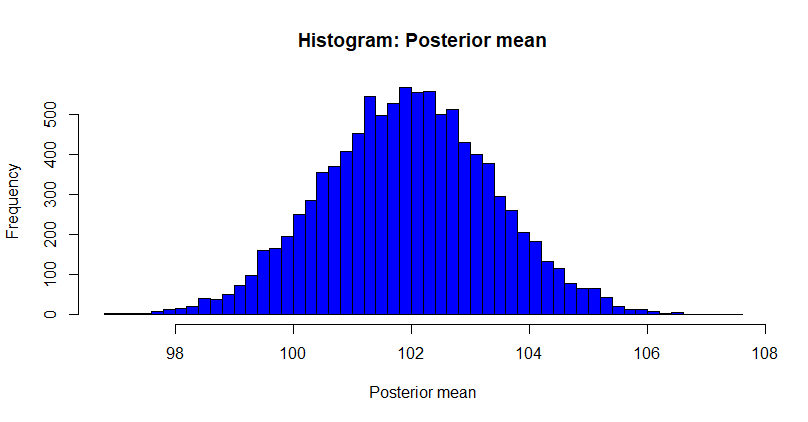
\includegraphics[width=340pt, height=200pt]{Chapters/chapter5/figures/PostMeanMathTest.png}
	%%\centerline{\epsfig{/Chapters/chapter1/figures/cat.eps,width=.8\textheight,height=.4\textwidth}}
	\caption[List of figure caption goes here]{Histogram of posterior draws of mean: Math test}\label{fig51}
\end{figure}

Figure \ref{fig51} shows the histogram of the draws of the posterior mean of the math test results. The posterior mean and median are 101.94 and 101.95, and the 95\% credible interval is (99.14, 104.79).\\

\end{enumerate}